\documentclass[11pt,usenames,dvipsnames,a4paper,twoside]{article}
\usepackage[T1]{fontenc}
% \usepackage{helvet}
% \renewcommand{\familydefault}{\sfdefault}
\usepackage[utf8]{inputenc}
\usepackage[spanish, es-tabla]{babel}
\usepackage{mathtools}
\usepackage{amsthm}
\usepackage{amsmath}
\usepackage{amsfonts}
\usepackage{amssymb}
\usepackage{makeidx}
\usepackage{graphicx}
\usepackage[table,xcdraw]{xcolor}
\usepackage{wrapfig}
\usepackage{lmodern}
\usepackage{tikz}
\usepackage{subcaption}
\usetikzlibrary{arrows,shapes,positioning,calc,babel}
\usepackage{pgfkeys} % LATEX
\usepackage{pgffor}
\usepackage{adjustbox}
\usepackage{fancybox}
\usepackage{pgfplots}
\pgfplotsset{compat=newest}
\usepackage{bm}
\usepackage{pdfpages}
\usepackage{siunitx}
\usepackage{multicol}
\usepackage{afterpage}
\usepackage{float}
\usepackage{xfrac}
\usepackage{hyperref}
\usepackage[italicdiff]{physics}
\usepackage[bottom=2.5cm, top = 2.5cm, right=2.5cm, left=2.5cm, bindingoffset=1cm]{geometry}

% \setlength{\parindent}{3em}
% \setlength{\parskip}{1em}

\begin{document}

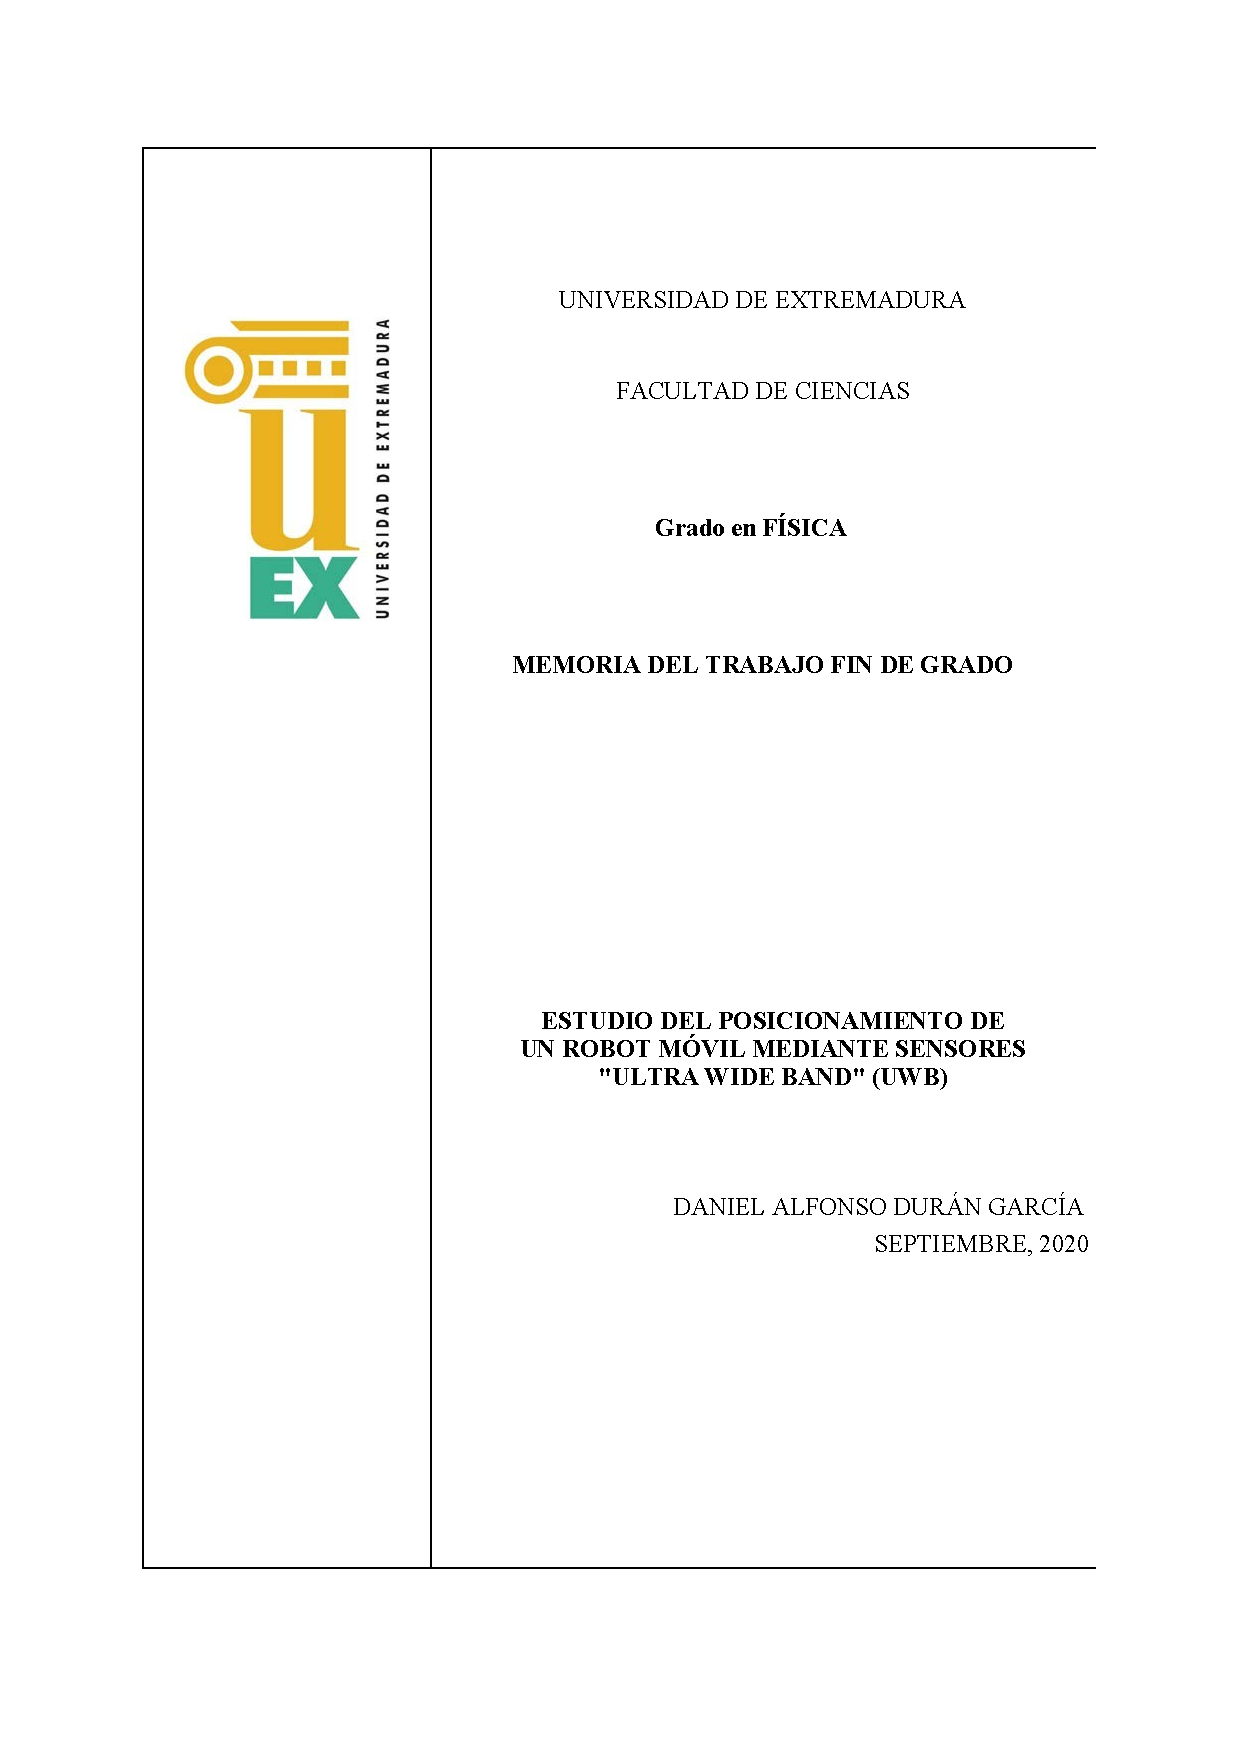
\includepdf[pages=1]{portada.pdf}

\shipout\null %Página en blanco

\pagestyle{empty}
\vspace*{5cm}

Carlos Javier García Orellana, profesor del
Departamento de Ingeniería Eléctrica, Electrónica y Automática de la Universidad de
Extremadura.

INFORMA:

Que D. Daniel Alfonso Durán García ha realizado
bajo su dirección el Trabajo Fin de Grado. Consideran que la memoria reúne
los requisitos necesarios para su evaluación.

\vspace*{1cm}
\begin{center}
Badajoz, día de mes de 2020


\vspace{5cm}
Fdo. Carlos Javier García Orellana
\end{center}

\newpage %Página en blanco
\setcounter{page}{1}
\pagestyle{plain}

\tableofcontents


%------------------------------------------------------------------------------
%                             Resumen
%------------------------------------------------------------------------------

\newpage
\section{Resumen}

%------------------------------------------------------------------------------
%                             Abstract
%------------------------------------------------------------------------------

\newpage
\section{Abstract}

%------------------------------------------------------------------------------
%                             Introduccion
%------------------------------------------------------------------------------

\newpage
\section{Introducción}

%------------------------------------------------------------------------------
%                             Metodologia
%------------------------------------------------------------------------------

\newpage
\section{Metodología}

%------------------------------------------------------------------------------
%                             Resultados
%------------------------------------------------------------------------------

\newpage
\section{Resultados}

%------------------------------------------------------------------------------
%                             Conclusiones
%------------------------------------------------------------------------------

\newpage
\section{Conclusiones}

\end{document}